% !TEX root = presentation.tex
\section{Introduction}
\subsection{Test Suite Effectiveness}
\frame{\frametitle{Test Suite Effectiveness}
  \begin{itemize}
    \item An effective test suite is \textit{``\ldots one that is capable of \alert{detecting all real bugs}''}~\footcite{Wey93}.
    \item Can measure \alert{code coverage} (e.g., branch, statement, path) being exercised by a test suite~\footcite{ZHM97}
    \item A more \alert{effective} determination of test suite effectiveness is \alert{mutation testing}.
  \end{itemize}
}

\subsection{Mutation Testing Overview}
\frame{\frametitle{Mutation Testing Overview}
  \begin{figure}[!tb]
    \centering
    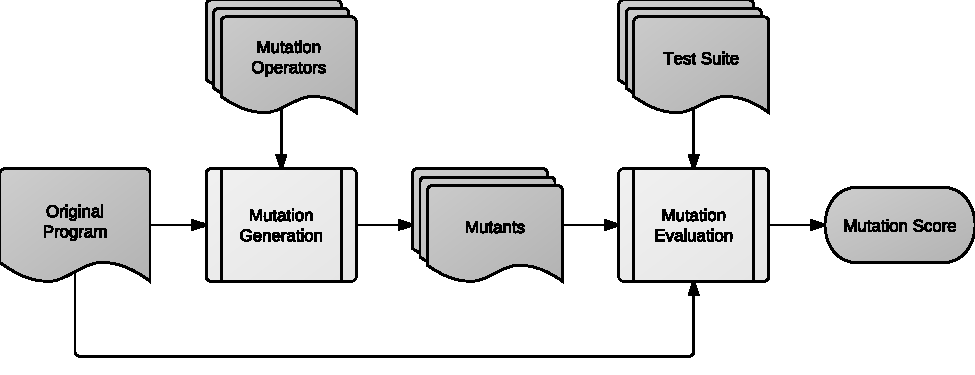
\includegraphics[width=\textwidth]{../thesis/figures/mutation_testing_overview.pdf}
    \caption{The mutation testing process.}
    \label{fig:mutation_testing_overview}
  \end{figure}
  \hrule
  \vspace{5mm}
  \begin{equation}
    \textit{$\text{mutation score} = \frac{\text{killed mutants}}{\text{total mutants} - \text{equivalent mutants}}$}
    \label{equ:mutation_score}
  \end{equation}
}

\subsubsection{Mutation Operator Example}
\frame{\frametitle{Mutation Operator Example (\textit{ROR})}
  \begin{figure}[!tb]
    \centering
    \begin{minipage}{4.75cm}
      \centering
      \footnotesize{\textbf{Original Program}}
      \lstinputlisting[language=Java, literate={>}{{\textcolor{red}{>}}}{1}]{../thesis/listings/mutation_example.java}
    \end{minipage}
    $\xrightarrow{\textit{ROR}}$
    \begin{minipage}{4.75cm}
      \centering
      \footnotesize{\textbf{Mutant Program}}
      \lstinputlisting[language=Java, literate={>}{{\textcolor{red}{<}}}{1}]{../thesis/listings/mutation_example.java}
    \end{minipage}
    \caption{Example application of the \alert{Relational Operator Replacement \textit{(ROR)}} method-level mutation operator.}
    \vspace{2mm}
    \hrule
    \label{fig:ROR_mutation}
  \end{figure}
  \begin{itemize}
    \item \alert{Hundreds or thousands} of mutants can be generated for even \alert{small} software systems.
  \end{itemize}
}
